%%%%%%%%%%%%%%%%%%%%%%%%%%%%%%%%%%%%%%%%%%%%%%%%%%%%%%%%%%%%%%%%%%%%%%%%%%%%%%%%%
%																				%
%	TRABAJO:	Trabajo Final													%
%				Especialidad en Ingenier�a en Sistemas de Informaci�n			%
%																				%
%		Titulo:																	%
%																				%
%		Autores:	Julian Nonino												%
%																				%
%	Capitulo sobre Apache Kafka													%	
%																				%
%	A�o: 2016																	%
%																				%
%%%%%%%%%%%%%%%%%%%%%%%%%%%%%%%%%%%%%%%%%%%%%%%%%%%%%%%%%%%%%%%%%%%%%%%%%%%%%%%%%

\chapter{Apache Kafka}
\label{chapter_apache_kafka}

Kafka es un sistema de mensajes distribuido, particionado y con
replicaci�n\cite{ApacheKafka090}.

\begin{itemize}
    \item Kafka mantiene los mensajes agrupados en categor�as llamadas
    \emph{topics.}
	\item Los productores de mensajes se llaman \emph{producers}.
	\item Los consumidores de mensajes se llaman \emph{consumers}.
	\item Kafka corre en un cluster formado por uno o mas servidores. cada uno de
	ellos es llamado \emph{broker}.
\end{itemize}

\begin{figure}[H]
	\centering
	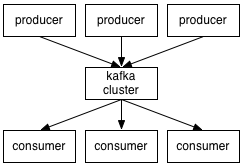
\includegraphics[width=.5\linewidth]{./marco_teorico/img/kafka/high_level_arch}
	\caption{Kafka, arquitectura de alto nivel\cite{ApacheKafka090}}
\end{figure}

\section{Topics}

	Los \emph{topics} de Kafka son categor�as de mensajes para los cuales Kafka
	mantiene registros particionados.
	
	Cada partici�n es una secuencia ordenada e inmutable de mensajes. El n�mero de
	orden de cada mensaje es llamado \emph{offset} e identifica univocamente a cada
	mensaje de la partici�n.
	
	Kafka mantiene los mensajes publicados por un per�odo de tiempo configurable,
	sin importar si fueron consumidos o no por alg�n proceso \emph{consumer}. Cada
	consumidor se encarga de mantener el \emph{offset} y tiene libertad para ir
	hacia atr�s y hacia adelante en los mensajes publicados para procesarlos.
	
	El tener los mensajes de un \emph{topic} particionados permite separar el
	\emph{topic} en varios servidores. �sto permite manejar grandes volumenes de
	datos y adem�s otorogar un nivel superior de paralelismo.
	
	\begin{figure}[H]
		\centering
		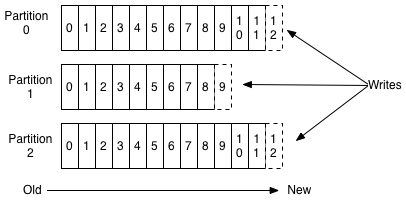
\includegraphics[width=.5\linewidth]{./marco_teorico/img/kafka/kafka_topics}
		\caption{Topics en Kafka\cite{ApacheKafka090}}
	\end{figure}
	
	Cada partici�n est� formada por un l�der (\emph{leader}) que se encuentra en
	uno de los servidores y por cero o m�s seguidores (\emph{followers}) que
	replican al l�der todo el tiempo en servidores distintos. Si el l�der falla,
	alguno de los seguidores se convertir� en el nuevo l�der garantizando que el
	sistema siga operando. la configuraci�n ideal es que cada servidor sea l�der de
	alguna partici�n y seguidor de las otras.
	
\section{Productores}
	
	Los productores en Kafka son programas encargados de publicar datos en los
	\emph{topics}. El productor decide, para cada mensaje, el topic y la partici�n
	en el cual publicarlo. Generalmente la partici�n es elegida siguiendo un
	esquema \emph{round-robin} para lograr un �ptimo balance de carga entre
	particiones, pero se puede utilizar cualquier l�gica.
	
\section{Consumidores}

	Los sitemas de mensajer�a pueden ser clasificados en dos categor�as,
	\emph{cola de mensajes} o \emph{publicaci�n-subscripci�n}. En el primero, los
	mensajes son encolados y cada mensaje es dirigido hacia alguno de los
	consumidores. En el segundo, cada mensaje es transmitido a todos los
	consumidores. kafka maneja ambos mundos con lo que se conoce como grupos de
	consumidores (\emph{consumer groups}).
	
	Cada consumidor debe ubicarse dentro de alguno de los grupos de consumidores y
	cuando un mensajes es publicado en un \emph{topic}, el mensaje es transmitido a
	un �nico consumidor de cada uno de los grupos de consumidores.
	
	\begin{figure}[H]
		\centering
		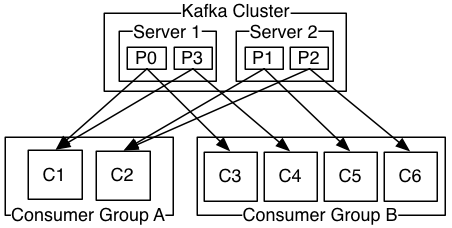
\includegraphics[width=.5\linewidth]{./marco_teorico/img/kafka/kafka_consumers}
		\caption{Grupos de Consumidores\cite{ApacheKafka090}}
	\end{figure}
	
	Si todos los consumidores se encuentran en el mismo grupo, el sistema funciona
	como una cola de mensajes distribuyendo la carga entre cada uno de los
	consumidores.
	
	Si todos los consumidores se encuentran en distintos grupos, el sistema
	funciona como un sistema publicaci�n-subscripci�n y todos los mensajes son
	transmitidos a todos los consumidores.
	
\section{Material}

	La informaci�n de �ste cap�tulo ha sido extra�da mayormente desde la
	documentaci�n de Apache Kafka 0.9 \cite{ApacheKafka090}.	